\documentclass[10pt,twocolumn,letterpaper]{article}
% ICCV Rules:
% 8 page limit (6 free + 2 paid)
% 10MB pdf file size limit
% 30MB supplementary materials file size limit (PDF or ZIP)

\usepackage{cvpr}
\usepackage[pagebackref=true,breaklinks=true,letterpaper=true,colorlinks,bookmarks=false]{hyperref}
\usepackage{times}
\usepackage{epsfig}
\usepackage{graphicx}
\usepackage{amsmath}
\usepackage{amssymb}
\usepackage{amsfonts}
\usepackage{algorithm}
\usepackage{algorithmic}
\usepackage{subfigure}

% Needed for getting formulas in dia diagrams.
\usepackage{pstricks}
\usepackage{tikz}

\usepackage{mydefs}

% \cvprfinalcopy % *** Uncomment this line for the final submission

\def\cvprPaperID{184} % *** Enter the CVPR Paper ID here
\def\httilde{\mbox{\tt\raisebox{-.5ex}{\symbol{126}}}}

% Pages are numbered in submission mode, and unnumbered in camera-ready

\hyphenation{under-determined}
\ifcvprfinal\pagestyle{empty}\fi
\begin{document}

%\title{Accelerating $\ell_1$-Minimization Using Many-Core CPUs/GPUs \\ and Application to Face Recognition
%\title{Efficient Parallelization of Sparse Representation for Face Recognition}
%\thanks{Corresponding author: . This work was partially supported by ARO MURI W911NF-06-1-0076.}}
%\title{Many-Core Parallelization of $\ell_1$-Minimization for Face Recognition
\title{\vspace{-0.2in} Parallelization of Fast $\ell_1$-Minimization for Face Recognition}
%\title{Parallelization of Fast $\ell_1$-Minimization Towards Real-Time Face Recognition}

\author{First Author\\
Institution1\\
Institution1 address\\
{\tt\small firstauthor@i1.org}
% For a paper whose authors are all at the same institution,
% omit the following lines up until the closing ``}''.
% Additional authors and addresses can be added with ``\and'',
% just like the second author.
% To save space, use either the email address or home page, not both
\and
Second Author\\
Institution2\\
First line of institution2 address\\
{\small\url{http://www.author.org/~second}}
}

\maketitle

\begin{abstract} Recently a family of promising face recognition algorithms
based on sparse representation and $\ell_1$-minimization ($\ell_1$-min) have been
developed.  These algorithms have not yet seen commercial application, 
largely due to higher computational cost compared to other traditional
algorithms. This paper studies techniques for leveraging the 
massive parallelism available in GPU and CPU hardware to accelerate
$\ell_1$-min based on augmented Lagrangian method (ALM) solvers. 
For very large problems, the GPU is faster due to higher memory bandwidth, while 
for problems that fit in the larger CPU L3 cache, the CPU is faster.
On both architectures, the proposed implementations significantly outperform
naive library-based implementations, as well as previous systems. 
The source code of the
algorithms will be made available for peer evaluation.  \end{abstract}
\vspace{-0.1in}

\section{Introduction} 
\vspace{-0.05in}
$\ell_1$-minimization ($\ell_1$-min) has received much attention in recent
years due to important applications in compressive sensing
\cite{BrucksteinA2007} and sparse representation \cite{WrightJ2010-PIEEE}.  
The problem refers to finding the minimum $\ell_1$-norm solution to an
underdetermined linear system $\bb=A\xx$:
\begin{equation}
\min \|\xx\|_1\quad \mbox{ subj. to }\quad \bb = A\xx.
\label{eq:l1min}
\end{equation}
It is now well established that, under certain conditions
\cite{CandesE2005-IT_1,DonohoD2004}, the minimum $\ell_1$-norm solution is also
the \emph{sparsest} solution to the system \eqref{eq:l1min}.

Among its many applications, $\ell_1$-min has been recently used to reformulate
image-based face recognition as a sparse representation problem
\cite{WrightJ2009-PAMI}.  If we stack the pixels of the training images of $K$ subject
classes into the columns of matrices $(A_1\in\Re^{d\times n_1}, \cdots, A_K\in\Re^{d\times n_K})$, combine
the matrices into a larger matrix $A = [A_1, \cdots, A_K]\in\Re^{d\times n}$, and arrange the pixels of a new
query image into a vector $\bb\in\Re^d$, \emph{sparsity-based
classification} (SBC) solves the following minimization problem:
\begin{equation}
\min_{\xx, \ee} \| \xx \|_1 + \|\ee\|_1 \quad \subj \quad \bb = A \xx + \ee.
\label{eq:l1min_denoise}
\end{equation}
If the sparsest solutions for $\x$ and $\e$ are recovered, $\ee$ provides a
means to compensate for pixels that are corrupted due to occlusion of some part of the query
image, and the dominant nonzero coefficients of $\xx$ reveal the membership of
$\bb$ based on the training image labels associated with $A$. 
%Since $A$ contains many images per user taken under different illuminations, 
%$A_i\x_i$ acts as a linear illumination model for the test image $\bb$.

In this paper, we study parallelization of $\ell$-min on many-core CPU and GPU
architectures. Although $\ell_1$-min \eqref{eq:l1min} is a convex
program, conventional algorithms such as interior-point methods
\cite{ChenS2001-SIAM,TibshiraniR1996} scale poorly
for applications such as face recognition. Recently, a number of
accelerated algorithms have been proposed that explicitly take advantage of
the special structure of $\ell_1$-min problems
\cite{LorisI2009,YangA2010-ICIP}. We investigate parallelization of a
state-of-the-art $\ell_1$-min solution based on
\emph{augmented Lagrangian methods} (ALM) \cite{BertsekasD2003,YangA2010-ICIP}.

In addition, the accuracy of the solution given by \eqref{eq:l1min_denoise} relies on the assumption
that the query image is well aligned with the training images.
In \cite{WagnerA2009-CVPR}, SBC was extended to align
a query image to each subject class individually. The alignment algorithm solves
the following problem:
\begin{equation}
\hat{\tau}_i = \arg\min_{\xx, \ee, \tau_i} \|\ee\|_1\quad \mbox{subj. to}\quad \tilde\bb\circ\tau_i = A_i\xx + \ee,
\label{eq:l1min_alignment}
\end{equation}
where $\tau_i\in T$ is in a finite-dimensional group $T$ of transformations
(e.g., affine or homography) acting on the image domain.  The sequence
$\tau_i$ converges to a transformation that aligns the test image $\tilde\bb$
with the training images from the $i$-th class $A_i$. In other words, the algorithm 
extends Lucas-Kanade iterative alignment \cite{LucasB1981} to use the
$\ell_1$-norm as a robust error function, while simultaneously estimating
the coefficients of the linear illumination model $A_i\x$.  

Although ALM has been applied to improve the speed of a prototype face recognition system \cite{WagnerA2011-PAMI},
due to the high per-class cost
of the alignment step, the system still fails to achieve \emph{real-time}
performance against datasets of hundreds or thousands of subjects.  In this paper,
in addition to accelerating the generic
$\ell_1$-min objectives \eqref{eq:l1min} and \eqref{eq:l1min_denoise}, we 
also discuss how to efficiently accelerate the face alignment step
\eqref{eq:l1min_alignment} on multi-core CPUs and GPUs.

To clarify discussion, we clearly distinguish between {\em parallelism},
which is a property of an algorithm, and {\em concurrency}, which is a
property of a hardware architecture. Parallelism in an algorithm provides the
opportunity to perform computations concurrently on hardware.  Algorithms often
exhibit multiple levels of parallelism, and hardware often provides multiple
levels of concurrency.  In these terms, the primary contribution of this paper
will be to determine the optimal mappings between the parallelism available in
$\ell_1$-min and the concurrency available in multi-core CPU and GPU
architectures.

Finally, we present extensive benchmark to compare the performance of the
generic ALM $\ell_1$-min algorithm and the corresponding face recognition
routines on massively parallel CPUs and GPUs.  To this end, a face
recognition system for security and access control applications has been implemented, 
and is diagrammed in Figure \ref{fig:pipeline}. This pipeline follows the work of \cite{WagnerA2011-PAMI}, but
the fast implementations presented in this paper are novel.
Since the parallelization of any algorithm
is highly dependent on the target hardware, we will give a brief overview of
the architecture of our test system in detail in Section
\ref{sec:concurrency}.
Finally, note that 
while this paper focuses on the parallelism available in a single (shared memory) machine,
applications targeting thousands of subjects or more will likely require computation to be
distributed over a cluster or network of computers. These systems are not addressed here.
The source code of our implementations, which target NVIDIA Fermi GPUs
as well as Intel x86-64 CPUs, will be made available for peer evaluation.
\begin{figure}
\centering
{\tiny % Graphic for TeX using PGF
% Title: pipeline_simplified.dia
% Creator: Dia v0.97-pre3
% CreationDate: Mon Feb 14 03:20:49 2011
% For: awagner
% \usepackage{tikz}
% The following commands are not supported in PSTricks at present
% We define them conditionally, so when they are implemented,
% this pgf file will use them.
\ifx\du\undefined
  \newlength{\du}
\fi
\setlength{\du}{15\unitlength}
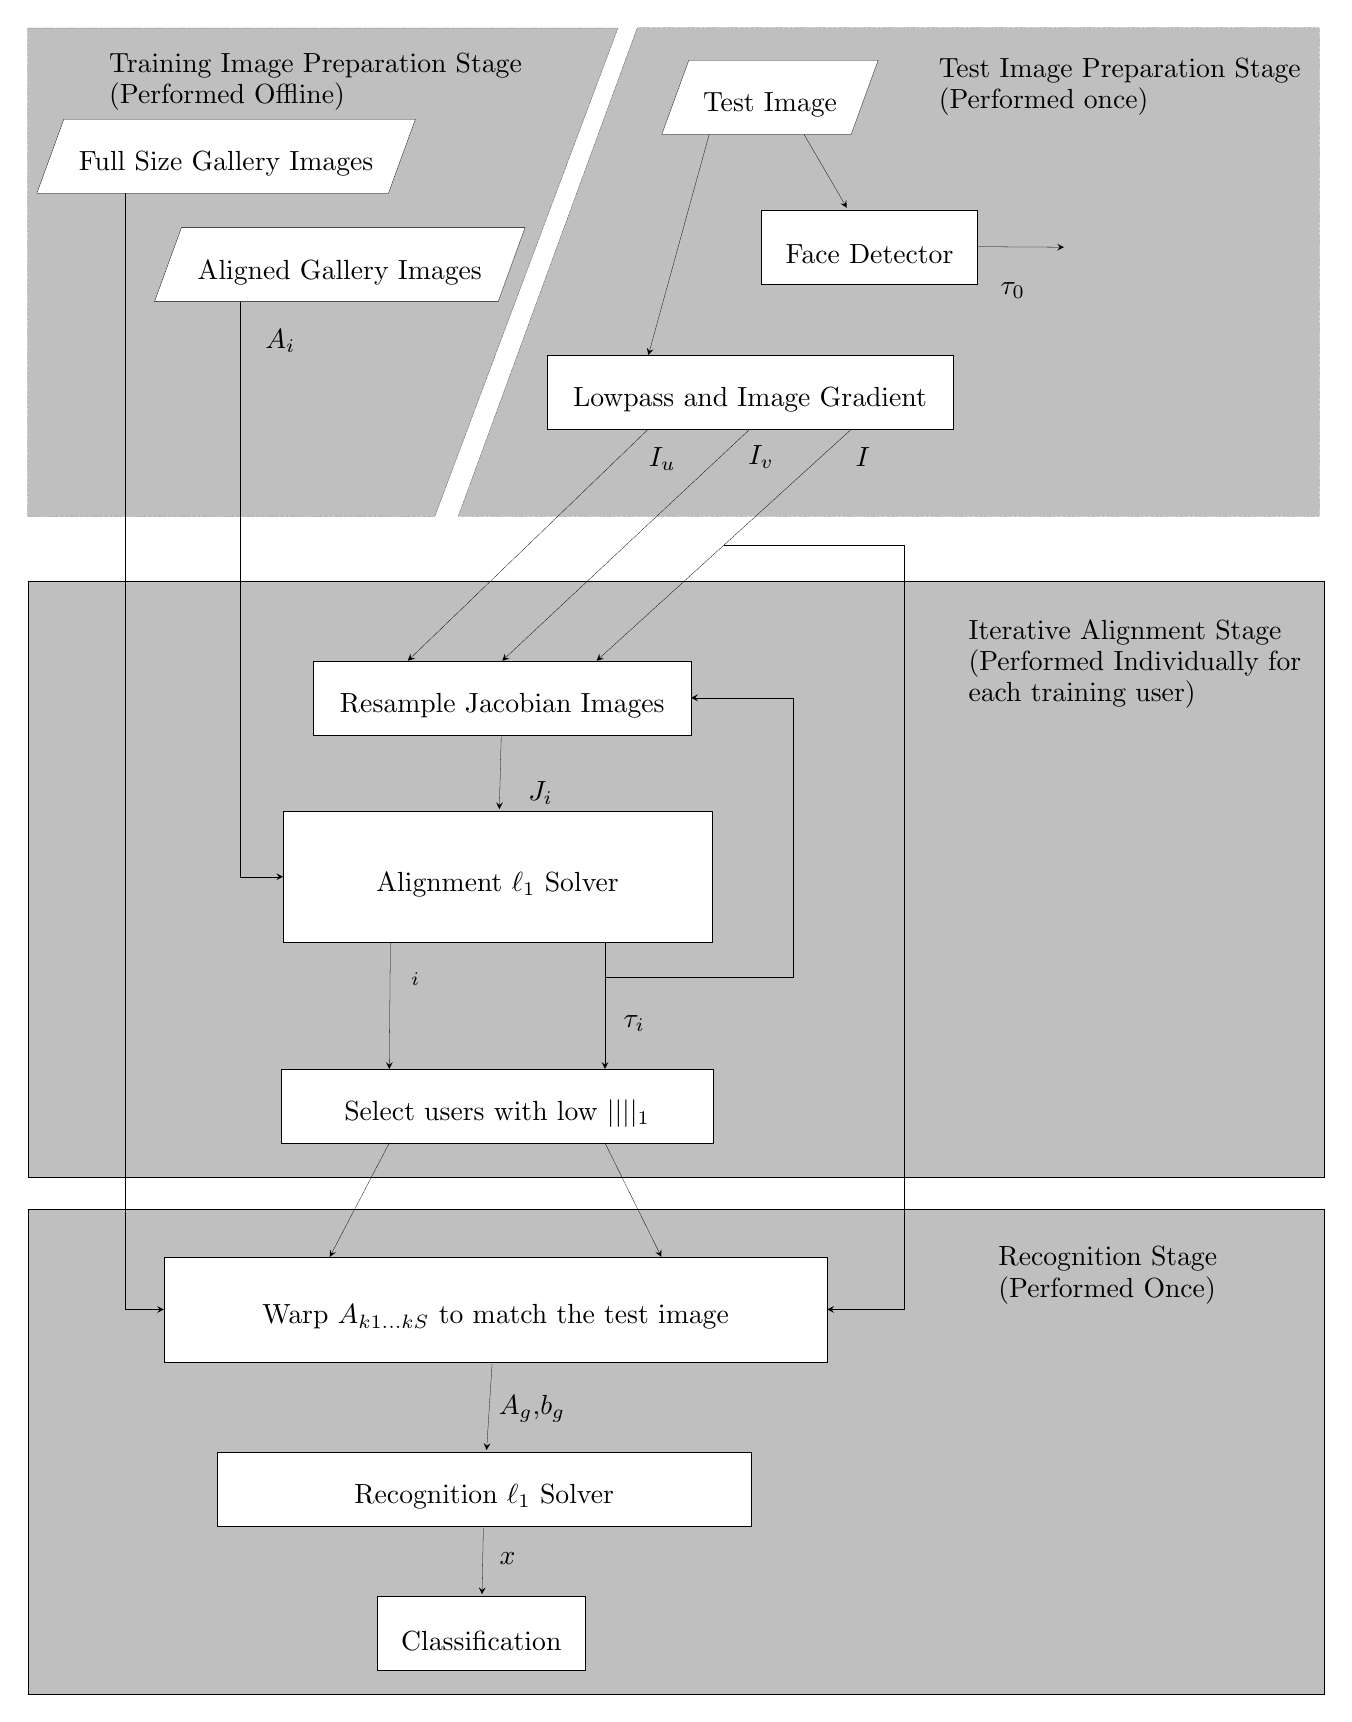
\begin{tikzpicture}
\pgftransformxscale{0.494667}
\pgftransformyscale{-0.494667}
\definecolor{dialinecolor}{rgb}{0.000000, 0.000000, 0.000000}
\pgfsetstrokecolor{dialinecolor}
\definecolor{dialinecolor}{rgb}{1.000000, 1.000000, 1.000000}
\pgfsetfillcolor{dialinecolor}
% setfont left to latex
\definecolor{dialinecolor}{rgb}{0.000000, 0.000000, 0.000000}
\pgfsetstrokecolor{dialinecolor}
\node[anchor=west] at (24.925000\du,42.952500\du){};
% setfont left to latex
\definecolor{dialinecolor}{rgb}{0.000000, 0.000000, 0.000000}
\pgfsetstrokecolor{dialinecolor}
\node[anchor=west] at (24.925000\du,42.952500\du){};
% setfont left to latex
\definecolor{dialinecolor}{rgb}{0.000000, 0.000000, 0.000000}
\pgfsetstrokecolor{dialinecolor}
\node[anchor=west] at (24.925000\du,42.952500\du){};
\definecolor{dialinecolor}{rgb}{0.749020, 0.749020, 0.749020}
\pgfsetfillcolor{dialinecolor}
\fill (6.494040\du,27.943300\du)--(6.494040\du,43.255071\du)--(39.770015\du,43.255071\du)--(39.770015\du,27.943300\du)--cycle;
\pgfsetlinewidth{0.100000\du}
\pgfsetdash{{\pgflinewidth}{0.200000\du}}{0cm}
\pgfsetdash{{\pgflinewidth}{0.200000\du}}{0cm}
\pgfsetmiterjoin
\definecolor{dialinecolor}{rgb}{0.000000, 0.000000, 0.000000}
\pgfsetstrokecolor{dialinecolor}
\draw (6.494040\du,27.943300\du)--(6.494040\du,43.255071\du)--(39.770015\du,43.255071\du)--(39.770015\du,27.943300\du)--cycle;
% setfont left to latex
\definecolor{dialinecolor}{rgb}{0.000000, 0.000000, 0.000000}
\pgfsetstrokecolor{dialinecolor}
\node at (23.132027\du,35.794186\du){};
\definecolor{dialinecolor}{rgb}{0.749020, 0.749020, 0.749020}
\pgfsetfillcolor{dialinecolor}
\fill (6.494040\du,44.061200\du)--(6.494040\du,56.519596\du)--(39.770015\du,56.519596\du)--(39.770015\du,44.061200\du)--cycle;
\pgfsetlinewidth{0.100000\du}
\pgfsetdash{{\pgflinewidth}{0.200000\du}}{0cm}
\pgfsetdash{{\pgflinewidth}{0.200000\du}}{0cm}
\pgfsetmiterjoin
\definecolor{dialinecolor}{rgb}{0.000000, 0.000000, 0.000000}
\pgfsetstrokecolor{dialinecolor}
\draw (6.494040\du,44.061200\du)--(6.494040\du,56.519596\du)--(39.770015\du,56.519596\du)--(39.770015\du,44.061200\du)--cycle;
% setfont left to latex
\definecolor{dialinecolor}{rgb}{0.000000, 0.000000, 0.000000}
\pgfsetstrokecolor{dialinecolor}
\node at (23.132027\du,50.485398\du){};
% setfont left to latex
\definecolor{dialinecolor}{rgb}{0.000000, 0.000000, 0.000000}
\pgfsetstrokecolor{dialinecolor}
\node[anchor=west] at (23.132000\du,35.599200\du){};
% setfont left to latex
\definecolor{dialinecolor}{rgb}{0.000000, 0.000000, 0.000000}
\pgfsetstrokecolor{dialinecolor}
\node[anchor=west] at (23.132000\du,35.599200\du){};
% setfont left to latex
\definecolor{dialinecolor}{rgb}{0.000000, 0.000000, 0.000000}
\pgfsetstrokecolor{dialinecolor}
\node[anchor=west] at (30.406100\du,29.259100\du){Iterative Alignment Stage};
% setfont left to latex
\definecolor{dialinecolor}{rgb}{0.000000, 0.000000, 0.000000}
\pgfsetstrokecolor{dialinecolor}
\node[anchor=west] at (30.406100\du,30.059100\du){(Performed Individually for};
% setfont left to latex
\definecolor{dialinecolor}{rgb}{0.000000, 0.000000, 0.000000}
\pgfsetstrokecolor{dialinecolor}
\node[anchor=west] at (30.406100\du,30.859100\du){each training user)};
% setfont left to latex
\definecolor{dialinecolor}{rgb}{0.000000, 0.000000, 0.000000}
\pgfsetstrokecolor{dialinecolor}
\node[anchor=west] at (31.173700\du,45.350700\du){Recognition Stage};
% setfont left to latex
\definecolor{dialinecolor}{rgb}{0.000000, 0.000000, 0.000000}
\pgfsetstrokecolor{dialinecolor}
\node[anchor=west] at (31.173700\du,46.150700\du){(Performed Once)};
\pgfsetlinewidth{0.100000\du}
\pgfsetdash{{\pgflinewidth}{0.200000\du}}{0cm}
\pgfsetdash{{\pgflinewidth}{0.200000\du}}{0cm}
\pgfsetmiterjoin
\pgfsetbuttcap
\definecolor{dialinecolor}{rgb}{0.749020, 0.749020, 0.749020}
\pgfsetfillcolor{dialinecolor}
\fill (6.494040\du,13.746400\du)--(21.645100\du,13.746400\du)--(16.943000\du,26.285100\du)--(6.494040\du,26.285100\du)--cycle;
\definecolor{dialinecolor}{rgb}{0.000000, 0.000000, 0.000000}
\pgfsetstrokecolor{dialinecolor}
\draw (6.494040\du,13.746400\du)--(21.645100\du,13.746400\du)--(16.943000\du,26.285100\du)--(6.494040\du,26.285100\du)--cycle;
% setfont left to latex
\definecolor{dialinecolor}{rgb}{0.000000, 0.000000, 0.000000}
\pgfsetstrokecolor{dialinecolor}
\node[anchor=west] at (8.342710\du,14.710900\du){Training Image Preparation Stage};
% setfont left to latex
\definecolor{dialinecolor}{rgb}{0.000000, 0.000000, 0.000000}
\pgfsetstrokecolor{dialinecolor}
\node[anchor=west] at (8.342710\du,15.510900\du){(Performed Offline)};
\pgfsetlinewidth{0.100000\du}
\pgfsetdash{{\pgflinewidth}{0.200000\du}}{0cm}
\pgfsetdash{{\pgflinewidth}{0.200000\du}}{0cm}
\pgfsetmiterjoin
\pgfsetbuttcap
\definecolor{dialinecolor}{rgb}{0.749020, 0.749020, 0.749020}
\pgfsetfillcolor{dialinecolor}
\fill (22.141100\du,13.740100\du)--(39.649500\du,13.740100\du)--(39.649500\du,26.278900\du)--(17.545800\du,26.278900\du)--cycle;
\definecolor{dialinecolor}{rgb}{0.000000, 0.000000, 0.000000}
\pgfsetstrokecolor{dialinecolor}
\draw (22.141100\du,13.740100\du)--(39.649500\du,13.740100\du)--(39.649500\du,26.278900\du)--(17.545800\du,26.278900\du)--cycle;
% setfont left to latex
\definecolor{dialinecolor}{rgb}{0.000000, 0.000000, 0.000000}
\pgfsetstrokecolor{dialinecolor}
\node[anchor=west] at (29.642500\du,14.831400\du){Test Image Preparation Stage};
% setfont left to latex
\definecolor{dialinecolor}{rgb}{0.000000, 0.000000, 0.000000}
\pgfsetstrokecolor{dialinecolor}
\node[anchor=west] at (29.642500\du,15.631400\du){(Performed once)};
\definecolor{dialinecolor}{rgb}{1.000000, 1.000000, 1.000000}
\pgfsetfillcolor{dialinecolor}
\fill (23.464443\du,14.572100\du)--(28.325620\du,14.572100\du)--(27.634076\du,16.472100\du)--(22.772900\du,16.472100\du)--cycle;
\pgfsetlinewidth{0.100000\du}
\pgfsetdash{}{0pt}
\pgfsetdash{}{0pt}
\pgfsetmiterjoin
\definecolor{dialinecolor}{rgb}{0.000000, 0.000000, 0.000000}
\pgfsetstrokecolor{dialinecolor}
\draw (23.464443\du,14.572100\du)--(28.325620\du,14.572100\du)--(27.634076\du,16.472100\du)--(22.772900\du,16.472100\du)--cycle;
% setfont left to latex
\definecolor{dialinecolor}{rgb}{0.000000, 0.000000, 0.000000}
\pgfsetstrokecolor{dialinecolor}
\node at (25.549260\du,15.717100\du){Test Image};
\definecolor{dialinecolor}{rgb}{1.000000, 1.000000, 1.000000}
\pgfsetfillcolor{dialinecolor}
\fill (13.826900\du,29.990700\du)--(13.826900\du,31.890700\du)--(23.521900\du,31.890700\du)--(23.521900\du,29.990700\du)--cycle;
\pgfsetlinewidth{0.100000\du}
\pgfsetdash{}{0pt}
\pgfsetdash{}{0pt}
\pgfsetmiterjoin
\definecolor{dialinecolor}{rgb}{0.000000, 0.000000, 0.000000}
\pgfsetstrokecolor{dialinecolor}
\draw (13.826900\du,29.990700\du)--(13.826900\du,31.890700\du)--(23.521900\du,31.890700\du)--(23.521900\du,29.990700\du)--cycle;
% setfont left to latex
\definecolor{dialinecolor}{rgb}{0.000000, 0.000000, 0.000000}
\pgfsetstrokecolor{dialinecolor}
\node at (18.674400\du,31.135700\du){Resample Jacobian Images};
\definecolor{dialinecolor}{rgb}{1.000000, 1.000000, 1.000000}
\pgfsetfillcolor{dialinecolor}
\fill (13.050000\du,33.850000\du)--(13.050000\du,37.221200\du)--(24.058800\du,37.221200\du)--(24.058800\du,33.850000\du)--cycle;
\pgfsetlinewidth{0.100000\du}
\pgfsetdash{}{0pt}
\pgfsetdash{}{0pt}
\pgfsetmiterjoin
\definecolor{dialinecolor}{rgb}{0.000000, 0.000000, 0.000000}
\pgfsetstrokecolor{dialinecolor}
\draw (13.050000\du,33.850000\du)--(13.050000\du,37.221200\du)--(24.058800\du,37.221200\du)--(24.058800\du,33.850000\du)--cycle;
% setfont left to latex
\definecolor{dialinecolor}{rgb}{0.000000, 0.000000, 0.000000}
\pgfsetstrokecolor{dialinecolor}
\node at (18.554400\du,35.730600\du){Alignment $\ell_1$ Solver};
\pgfsetlinewidth{0.100000\du}
\pgfsetdash{}{0pt}
\pgfsetdash{}{0pt}
\pgfsetbuttcap
{
\definecolor{dialinecolor}{rgb}{0.000000, 0.000000, 0.000000}
\pgfsetfillcolor{dialinecolor}
% was here!!!
\pgfsetarrowsend{stealth}
\definecolor{dialinecolor}{rgb}{0.000000, 0.000000, 0.000000}
\pgfsetstrokecolor{dialinecolor}
\draw (18.648326\du,31.939104\du)--(18.599693\du,33.801294\du);
}
% setfont left to latex
\definecolor{dialinecolor}{rgb}{0.000000, 0.000000, 0.000000}
\pgfsetstrokecolor{dialinecolor}
\node[anchor=west] at (11.250000\du,34.890000\du){};
\definecolor{dialinecolor}{rgb}{1.000000, 1.000000, 1.000000}
\pgfsetfillcolor{dialinecolor}
\fill (19.817600\du,22.143000\du)--(19.817600\du,24.043000\du)--(30.250100\du,24.043000\du)--(30.250100\du,22.143000\du)--cycle;
\pgfsetlinewidth{0.100000\du}
\pgfsetdash{}{0pt}
\pgfsetdash{}{0pt}
\pgfsetmiterjoin
\definecolor{dialinecolor}{rgb}{0.000000, 0.000000, 0.000000}
\pgfsetstrokecolor{dialinecolor}
\draw (19.817600\du,22.143000\du)--(19.817600\du,24.043000\du)--(30.250100\du,24.043000\du)--(30.250100\du,22.143000\du)--cycle;
% setfont left to latex
\definecolor{dialinecolor}{rgb}{0.000000, 0.000000, 0.000000}
\pgfsetstrokecolor{dialinecolor}
\node at (25.033850\du,23.288000\du){Lowpass and Image Gradient};
\definecolor{dialinecolor}{rgb}{1.000000, 1.000000, 1.000000}
\pgfsetfillcolor{dialinecolor}
\fill (25.332900\du,18.409900\du)--(25.332900\du,20.309900\du)--(30.875400\du,20.309900\du)--(30.875400\du,18.409900\du)--cycle;
\pgfsetlinewidth{0.100000\du}
\pgfsetdash{}{0pt}
\pgfsetdash{}{0pt}
\pgfsetmiterjoin
\definecolor{dialinecolor}{rgb}{0.000000, 0.000000, 0.000000}
\pgfsetstrokecolor{dialinecolor}
\draw (25.332900\du,18.409900\du)--(25.332900\du,20.309900\du)--(30.875400\du,20.309900\du)--(30.875400\du,18.409900\du)--cycle;
% setfont left to latex
\definecolor{dialinecolor}{rgb}{0.000000, 0.000000, 0.000000}
\pgfsetstrokecolor{dialinecolor}
\node at (28.104150\du,19.554900\du){Face Detector};
\definecolor{dialinecolor}{rgb}{1.000000, 1.000000, 1.000000}
\pgfsetfillcolor{dialinecolor}
\fill (9.987950\du,45.295200\du)--(9.987950\du,47.995200\du)--(27.017950\du,47.995200\du)--(27.017950\du,45.295200\du)--cycle;
\pgfsetlinewidth{0.100000\du}
\pgfsetdash{}{0pt}
\pgfsetdash{}{0pt}
\pgfsetmiterjoin
\definecolor{dialinecolor}{rgb}{0.000000, 0.000000, 0.000000}
\pgfsetstrokecolor{dialinecolor}
\draw (9.987950\du,45.295200\du)--(9.987950\du,47.995200\du)--(27.017950\du,47.995200\du)--(27.017950\du,45.295200\du)--cycle;
% setfont left to latex
\definecolor{dialinecolor}{rgb}{0.000000, 0.000000, 0.000000}
\pgfsetstrokecolor{dialinecolor}
\node at (18.502950\du,46.840200\du){Warp $A_{k1 \ldots kS}$ to match the test image};
\definecolor{dialinecolor}{rgb}{1.000000, 1.000000, 1.000000}
\pgfsetfillcolor{dialinecolor}
\fill (15.470400\du,54.006500\du)--(15.470400\du,55.906500\du)--(20.802900\du,55.906500\du)--(20.802900\du,54.006500\du)--cycle;
\pgfsetlinewidth{0.100000\du}
\pgfsetdash{}{0pt}
\pgfsetdash{}{0pt}
\pgfsetmiterjoin
\definecolor{dialinecolor}{rgb}{0.000000, 0.000000, 0.000000}
\pgfsetstrokecolor{dialinecolor}
\draw (15.470400\du,54.006500\du)--(15.470400\du,55.906500\du)--(20.802900\du,55.906500\du)--(20.802900\du,54.006500\du)--cycle;
% setfont left to latex
\definecolor{dialinecolor}{rgb}{0.000000, 0.000000, 0.000000}
\pgfsetstrokecolor{dialinecolor}
\node at (18.136650\du,55.151500\du){Classification};
% setfont left to latex
\definecolor{dialinecolor}{rgb}{0.000000, 0.000000, 0.000000}
\pgfsetstrokecolor{dialinecolor}
\node[anchor=west] at (28.104200\du,19.359900\du){};
\pgfsetlinewidth{0.100000\du}
\pgfsetdash{}{0pt}
\pgfsetdash{}{0pt}
\pgfsetbuttcap
{
\definecolor{dialinecolor}{rgb}{0.000000, 0.000000, 0.000000}
\pgfsetfillcolor{dialinecolor}
% was here!!!
\pgfsetarrowsend{stealth}
\definecolor{dialinecolor}{rgb}{0.000000, 0.000000, 0.000000}
\pgfsetstrokecolor{dialinecolor}
\draw (25.033800\du,24.043000\du)--(18.674400\du,29.990700\du);
}
\pgfsetlinewidth{0.100000\du}
\pgfsetdash{}{0pt}
\pgfsetdash{}{0pt}
\pgfsetbuttcap
{
\definecolor{dialinecolor}{rgb}{0.000000, 0.000000, 0.000000}
\pgfsetfillcolor{dialinecolor}
% was here!!!
\pgfsetarrowsend{stealth}
\definecolor{dialinecolor}{rgb}{0.000000, 0.000000, 0.000000}
\pgfsetstrokecolor{dialinecolor}
\draw (22.425700\du,24.043000\du)--(16.250600\du,29.990700\du);
}
\pgfsetlinewidth{0.100000\du}
\pgfsetdash{}{0pt}
\pgfsetdash{}{0pt}
\pgfsetbuttcap
{
\definecolor{dialinecolor}{rgb}{0.000000, 0.000000, 0.000000}
\pgfsetfillcolor{dialinecolor}
% was here!!!
\pgfsetarrowsend{stealth}
\definecolor{dialinecolor}{rgb}{0.000000, 0.000000, 0.000000}
\pgfsetstrokecolor{dialinecolor}
\draw (27.641900\du,24.043000\du)--(21.098100\du,29.990700\du);
}
% setfont left to latex
\definecolor{dialinecolor}{rgb}{0.000000, 0.000000, 0.000000}
\pgfsetstrokecolor{dialinecolor}
\node[anchor=west] at (27.506000\du,24.761200\du){$I$};
% setfont left to latex
\definecolor{dialinecolor}{rgb}{0.000000, 0.000000, 0.000000}
\pgfsetstrokecolor{dialinecolor}
\node[anchor=west] at (22.199300\du,24.802400\du){$I_u$};
\pgfsetlinewidth{0.100000\du}
\pgfsetdash{}{0pt}
\pgfsetdash{}{0pt}
\pgfsetbuttcap
{
\definecolor{dialinecolor}{rgb}{0.000000, 0.000000, 0.000000}
\pgfsetfillcolor{dialinecolor}
% was here!!!
\pgfsetarrowsend{stealth}
\definecolor{dialinecolor}{rgb}{0.000000, 0.000000, 0.000000}
\pgfsetstrokecolor{dialinecolor}
\draw (23.988200\du,16.472100\du)--(22.425700\du,22.143000\du);
}
\pgfsetlinewidth{0.100000\du}
\pgfsetdash{}{0pt}
\pgfsetdash{}{0pt}
\pgfsetbuttcap
{
\definecolor{dialinecolor}{rgb}{0.000000, 0.000000, 0.000000}
\pgfsetfillcolor{dialinecolor}
% was here!!!
\pgfsetarrowsend{stealth}
\definecolor{dialinecolor}{rgb}{0.000000, 0.000000, 0.000000}
\pgfsetstrokecolor{dialinecolor}
\draw (26.418800\du,16.472100\du)--(27.520491\du,18.359816\du);
}
% setfont left to latex
\definecolor{dialinecolor}{rgb}{0.000000, 0.000000, 0.000000}
\pgfsetstrokecolor{dialinecolor}
\node[anchor=west] at (28.248200\du,27.724100\du){};
% setfont left to latex
\definecolor{dialinecolor}{rgb}{0.000000, 0.000000, 0.000000}
\pgfsetstrokecolor{dialinecolor}
\node[anchor=west] at (31.230200\du,20.488200\du){$\tau_0$};
\definecolor{dialinecolor}{rgb}{1.000000, 1.000000, 1.000000}
\pgfsetfillcolor{dialinecolor}
\fill (7.418823\du,16.086600\du)--(16.445000\du,16.086600\du)--(15.753456\du,17.986600\du)--(6.727280\du,17.986600\du)--cycle;
\pgfsetlinewidth{0.100000\du}
\pgfsetdash{}{0pt}
\pgfsetdash{}{0pt}
\pgfsetmiterjoin
\definecolor{dialinecolor}{rgb}{0.000000, 0.000000, 0.000000}
\pgfsetstrokecolor{dialinecolor}
\draw (7.418823\du,16.086600\du)--(16.445000\du,16.086600\du)--(15.753456\du,17.986600\du)--(6.727280\du,17.986600\du)--cycle;
% setfont left to latex
\definecolor{dialinecolor}{rgb}{0.000000, 0.000000, 0.000000}
\pgfsetstrokecolor{dialinecolor}
\node at (11.586140\du,17.231600\du){Full Size Gallery Images};
\pgfsetlinewidth{0.100000\du}
\pgfsetdash{}{0pt}
\pgfsetdash{}{0pt}
\pgfsetmiterjoin
\pgfsetbuttcap
{
\definecolor{dialinecolor}{rgb}{0.000000, 0.000000, 0.000000}
\pgfsetfillcolor{dialinecolor}
% was here!!!
\pgfsetarrowsend{stealth}
{\pgfsetcornersarced{\pgfpoint{0.000000\du}{0.000000\du}}\definecolor{dialinecolor}{rgb}{0.000000, 0.000000, 0.000000}
\pgfsetstrokecolor{dialinecolor}
\draw (11.952169\du,20.770000\du)--(11.952169\du,35.535600\du)--(13.050000\du,35.535600\du);
}}
\pgfsetlinewidth{0.100000\du}
\pgfsetdash{}{0pt}
\pgfsetdash{}{0pt}
\pgfsetbuttcap
{
\definecolor{dialinecolor}{rgb}{0.000000, 0.000000, 0.000000}
\pgfsetfillcolor{dialinecolor}
% was here!!!
\pgfsetarrowsend{stealth}
\definecolor{dialinecolor}{rgb}{0.000000, 0.000000, 0.000000}
\pgfsetstrokecolor{dialinecolor}
\draw (30.875400\du,19.359900\du)--(33.098700\du,19.372700\du);
}
\definecolor{dialinecolor}{rgb}{1.000000, 1.000000, 1.000000}
\pgfsetfillcolor{dialinecolor}
\fill (11.356800\du,50.303600\du)--(11.356800\du,52.203600\du)--(25.061036\du,52.203600\du)--(25.061036\du,50.303600\du)--cycle;
\pgfsetlinewidth{0.100000\du}
\pgfsetdash{}{0pt}
\pgfsetdash{}{0pt}
\pgfsetmiterjoin
\definecolor{dialinecolor}{rgb}{0.000000, 0.000000, 0.000000}
\pgfsetstrokecolor{dialinecolor}
\draw (11.356800\du,50.303600\du)--(11.356800\du,52.203600\du)--(25.061036\du,52.203600\du)--(25.061036\du,50.303600\du)--cycle;
% setfont left to latex
\definecolor{dialinecolor}{rgb}{0.000000, 0.000000, 0.000000}
\pgfsetstrokecolor{dialinecolor}
\node at (18.208918\du,51.448600\du){Recognition $\ell_1$ Solver};
\pgfsetlinewidth{0.100000\du}
\pgfsetdash{}{0pt}
\pgfsetdash{}{0pt}
\pgfsetmiterjoin
\pgfsetbuttcap
{
\definecolor{dialinecolor}{rgb}{0.000000, 0.000000, 0.000000}
\pgfsetfillcolor{dialinecolor}
% was here!!!
\pgfsetarrowsend{stealth}
{\pgfsetcornersarced{\pgfpoint{0.000000\du}{0.000000\du}}\definecolor{dialinecolor}{rgb}{0.000000, 0.000000, 0.000000}
\pgfsetstrokecolor{dialinecolor}
\draw (21.306600\du,37.221200\du)--(21.306600\du,38.050000\du)--(21.312500\du,38.050000\du)--(21.312500\du,40.470000\du);
}}
\pgfsetlinewidth{0.100000\du}
\pgfsetdash{}{0pt}
\pgfsetdash{}{0pt}
\pgfsetbuttcap
{
\definecolor{dialinecolor}{rgb}{0.000000, 0.000000, 0.000000}
\pgfsetfillcolor{dialinecolor}
% was here!!!
\pgfsetarrowsend{stealth}
\definecolor{dialinecolor}{rgb}{0.000000, 0.000000, 0.000000}
\pgfsetstrokecolor{dialinecolor}
\draw (15.802200\du,37.221200\du)--(15.775000\du,40.470000\du);
}
% setfont left to latex
\definecolor{dialinecolor}{rgb}{0.000000, 0.000000, 0.000000}
\pgfsetstrokecolor{dialinecolor}
\node[anchor=west] at (16.096600\du,38.150600\du){$\e_i$};
\pgfsetlinewidth{0.100000\du}
\pgfsetdash{}{0pt}
\pgfsetdash{}{0pt}
\pgfsetbuttcap
{
\definecolor{dialinecolor}{rgb}{0.000000, 0.000000, 0.000000}
\pgfsetfillcolor{dialinecolor}
% was here!!!
\pgfsetarrowsend{stealth}
\definecolor{dialinecolor}{rgb}{0.000000, 0.000000, 0.000000}
\pgfsetstrokecolor{dialinecolor}
\draw (18.189395\du,52.253907\du)--(18.156173\du,53.956193\du);
}
\pgfsetlinewidth{0.100000\du}
\pgfsetdash{}{0pt}
\pgfsetdash{}{0pt}
\pgfsetmiterjoin
\pgfsetbuttcap
{
\definecolor{dialinecolor}{rgb}{0.000000, 0.000000, 0.000000}
\pgfsetfillcolor{dialinecolor}
% was here!!!
\pgfsetarrowsend{stealth}
{\pgfsetcornersarced{\pgfpoint{0.000000\du}{0.000000\du}}\definecolor{dialinecolor}{rgb}{0.000000, 0.000000, 0.000000}
\pgfsetstrokecolor{dialinecolor}
\draw (24.370000\du,27.016800\du)--(28.999500\du,27.016800\du)--(28.999500\du,46.645200\du)--(27.018000\du,46.645200\du);
}}
\pgfsetlinewidth{0.100000\du}
\pgfsetdash{}{0pt}
\pgfsetdash{}{0pt}
\pgfsetbuttcap
{
\definecolor{dialinecolor}{rgb}{0.000000, 0.000000, 0.000000}
\pgfsetfillcolor{dialinecolor}
% was here!!!
\pgfsetarrowsend{stealth}
\definecolor{dialinecolor}{rgb}{0.000000, 0.000000, 0.000000}
\pgfsetstrokecolor{dialinecolor}
\draw (18.413613\du,48.045384\du)--(18.272699\du,50.253951\du);
}
% setfont left to latex
\definecolor{dialinecolor}{rgb}{0.000000, 0.000000, 0.000000}
\pgfsetstrokecolor{dialinecolor}
\node[anchor=west] at (18.367000\du,53.041300\du){$x$};
% setfont left to latex
\definecolor{dialinecolor}{rgb}{0.000000, 0.000000, 0.000000}
\pgfsetstrokecolor{dialinecolor}
\node[anchor=west] at (18.349600\du,49.203000\du){$A_g$,$b_g$};
% setfont left to latex
\definecolor{dialinecolor}{rgb}{0.000000, 0.000000, 0.000000}
\pgfsetstrokecolor{dialinecolor}
\node[anchor=west] at (24.755000\du,24.750000\du){$I_v$};
% setfont left to latex
\definecolor{dialinecolor}{rgb}{0.000000, 0.000000, 0.000000}
\pgfsetstrokecolor{dialinecolor}
\node[anchor=west] at (12.355000\du,21.787500\du){$A_i$};
% setfont left to latex
\definecolor{dialinecolor}{rgb}{0.000000, 0.000000, 0.000000}
\pgfsetstrokecolor{dialinecolor}
\node[anchor=west] at (19.105000\du,33.387500\du){$J_i$};
\definecolor{dialinecolor}{rgb}{1.000000, 1.000000, 1.000000}
\pgfsetfillcolor{dialinecolor}
\fill (10.437793\du,18.870000\du)--(19.261470\du,18.870000\du)--(18.569926\du,20.770000\du)--(9.746250\du,20.770000\du)--cycle;
\pgfsetlinewidth{0.100000\du}
\pgfsetdash{}{0pt}
\pgfsetdash{}{0pt}
\pgfsetmiterjoin
\definecolor{dialinecolor}{rgb}{0.000000, 0.000000, 0.000000}
\pgfsetstrokecolor{dialinecolor}
\draw (10.437793\du,18.870000\du)--(19.261470\du,18.870000\du)--(18.569926\du,20.770000\du)--(9.746250\du,20.770000\du)--cycle;
% setfont left to latex
\definecolor{dialinecolor}{rgb}{0.000000, 0.000000, 0.000000}
\pgfsetstrokecolor{dialinecolor}
\node at (14.503860\du,20.015000\du){Aligned Gallery Images};
\pgfsetlinewidth{0.100000\du}
\pgfsetdash{}{0pt}
\pgfsetdash{}{0pt}
\pgfsetmiterjoin
\pgfsetbuttcap
{
\definecolor{dialinecolor}{rgb}{0.000000, 0.000000, 0.000000}
\pgfsetfillcolor{dialinecolor}
% was here!!!
\pgfsetarrowsend{stealth}
{\pgfsetcornersarced{\pgfpoint{0.000000\du}{0.000000\du}}\definecolor{dialinecolor}{rgb}{0.000000, 0.000000, 0.000000}
\pgfsetstrokecolor{dialinecolor}
\draw (8.983824\du,17.986600\du)--(8.983824\du,46.645200\du)--(9.987950\du,46.645200\du);
}}
\pgfsetlinewidth{0.100000\du}
\pgfsetdash{}{0pt}
\pgfsetdash{}{0pt}
\pgfsetmiterjoin
\pgfsetbuttcap
{
\definecolor{dialinecolor}{rgb}{0.000000, 0.000000, 0.000000}
\pgfsetfillcolor{dialinecolor}
% was here!!!
\pgfsetarrowsend{stealth}
{\pgfsetcornersarced{\pgfpoint{0.000000\du}{0.000000\du}}\definecolor{dialinecolor}{rgb}{0.000000, 0.000000, 0.000000}
\pgfsetstrokecolor{dialinecolor}
\draw (21.300000\du,38.100000\du)--(26.150000\du,38.100000\du)--(26.150000\du,30.940700\du)--(23.521900\du,30.940700\du);
}}
% setfont left to latex
\definecolor{dialinecolor}{rgb}{0.000000, 0.000000, 0.000000}
\pgfsetstrokecolor{dialinecolor}
\node[anchor=west] at (21.550000\du,39.300000\du){$\tau_i$};
\definecolor{dialinecolor}{rgb}{1.000000, 1.000000, 1.000000}
\pgfsetfillcolor{dialinecolor}
\fill (13.006200\du,40.470000\du)--(13.006200\du,42.370000\du)--(24.081200\du,42.370000\du)--(24.081200\du,40.470000\du)--cycle;
\pgfsetlinewidth{0.100000\du}
\pgfsetdash{}{0pt}
\pgfsetdash{}{0pt}
\pgfsetmiterjoin
\definecolor{dialinecolor}{rgb}{0.000000, 0.000000, 0.000000}
\pgfsetstrokecolor{dialinecolor}
\draw (13.006200\du,40.470000\du)--(13.006200\du,42.370000\du)--(24.081200\du,42.370000\du)--(24.081200\du,40.470000\du)--cycle;
% setfont left to latex
\definecolor{dialinecolor}{rgb}{0.000000, 0.000000, 0.000000}
\pgfsetstrokecolor{dialinecolor}
\node at (18.543700\du,41.615000\du){Select users with low $||\e||_1$};
\pgfsetlinewidth{0.100000\du}
\pgfsetdash{}{0pt}
\pgfsetdash{}{0pt}
\pgfsetbuttcap
{
\definecolor{dialinecolor}{rgb}{0.000000, 0.000000, 0.000000}
\pgfsetfillcolor{dialinecolor}
% was here!!!
\pgfsetarrowsend{stealth}
\definecolor{dialinecolor}{rgb}{0.000000, 0.000000, 0.000000}
\pgfsetstrokecolor{dialinecolor}
\draw (15.775000\du,42.370000\du)--(14.245500\du,45.295200\du);
}
\pgfsetlinewidth{0.100000\du}
\pgfsetdash{}{0pt}
\pgfsetdash{}{0pt}
\pgfsetbuttcap
{
\definecolor{dialinecolor}{rgb}{0.000000, 0.000000, 0.000000}
\pgfsetfillcolor{dialinecolor}
% was here!!!
\pgfsetarrowsend{stealth}
\definecolor{dialinecolor}{rgb}{0.000000, 0.000000, 0.000000}
\pgfsetstrokecolor{dialinecolor}
\draw (21.312500\du,42.370000\du)--(22.760500\du,45.295200\du);
}
\end{tikzpicture}
}
\caption{The face recognition pipeline.\vspace{-0.1in}}
\label{fig:pipeline}
\end{figure}


\subsection{Literature Review} \vspace{-0.05in}
Traditionally, $\ell_1$-min (a.k.a.
basis pursuit (BP)) has been formulated as a linear program
\cite{ChenS2001-SIAM}. Several variations of the solution are also well known
in optimization, including a noisy approximation via quadratic programming
called the LASSO \cite{TibshiraniR1996} and truncated Newton interior-point
method (TNIPM) \cite{KimS2007}.

One of the drawbacks of most interior-point methods for $\ell_1$-min is that they require the solution sequence to follow an
interior path via gradient descent or conjugate gradient methods, which are computationally expensive.
To mitigate these issues, an approach called \emph{Homotopy} has been recently studied to accelerate the
speed of $\ell_1$-min \cite{OsborneM2000,EfronB2004,MalioutovD2005,DonohoD2006}.
Although Homotopy can be shown to exactly estimate BP when the solution is
sufficiently sparse \cite{DonohoD2006}, the algorithm still involves
computationally expensive operations such as matrix-matrix multiplication and
linear least-squares problems with varying $A$
matrices.

%Homotopy methods for recovering sparse signals were
%first studied in the context of LASSO \cite{OsborneM2000}, which inspired a
%solution to the \emph{forward stagewise linear regression} problem called LARS
%\cite{EfronB2004}, and eventually led to the corresponding Homotopy algorithms
%for BP in \cite{MalioutovD2005,DonohoD2006}.


%\footnote{During the face alignment algorithm presented later, The $A$ matrix changes between alignment iterations but not within the L1 solver}  
In Section \ref{sec:ALM}, we contend that ALM is a better choice for
implementation on many-core CPUs and GPUs. The ALM algorithm belongs to a
category of approximate $\ell_1$-min solutions called \emph{iterative
shrinkage-thresholding} (IST) methods \cite{WrightS2008,BeckA2009}.  IST
algorithms mainly involve elementary operations such as vector algebra and
matrix-vector multiplication. Therefore, when the dimension of the problem
becomes high, IST-type algorithms are particularly suitable for hardware
systems with a high degree of concurrency. In \cite{YangA2010-ICIP}, the
authors showed that ALM is able to significantly improve the solver speed,
while achieving estimation accuracy competitive with other $\ell_1$-min
solutions. Therefore, we choose ALM as the core algorithm for
implementation of $\ell_1$-min in the parallel face recognition pipeline.

In terms of the past works in parallel $\ell_1$-min, the literature has been
limited, to the best of our knowledge. In \cite{BorghiA2010}, Borghi et al.
developed a special proximal gradient $\ell_1$-min algorithm based on
Moreau-Yosida regularization. In \cite{MurphyM2010}, Murphy et al. presented
parallel implementation of the l1-SPIRIT MRI reconstruction algorithm on 
the same GPU architecture addressed in this paper.

\section{Augmented Lagrangian Method}
\label{sec:ALM}
\vspace{-0.05in}
In this section, we briefly describe the ALM algorithm for $\ell_1$-min
\eqref{eq:l1min} \cite{YangA2010-ICIP} and analyze its complexity. Lagrange
multipliers have been frequently used in convex programming to eliminate
equality constraints via adding a penalty term to the cost function for
infeasible points. ALM methods differ from other penalty-based approaches by
simultaneously estimating the optimal solution and Lagrange multipliers in an
iterative fashion.  For $\ell_1$-min \eqref{eq:l1min}, the augmented Lagrange
function is defined as: 
\begin{equation} L_\mu(\xx,\yy) = \|\xx\|_1 +
\yy^T(\bb - A\xx) + \frac{\mu}{2} \| \bb-A\xx \|_2^2, 
\end{equation}
where $\mu > 0$ is a constant that penalizes infeasibility and $\yy$ is a
vector of Lagrange multipliers.

In Lagrange Multiplier Theory \cite{BertsekasD2003}, if there exists a Lagrangian $y^*$ that
satisfies the second-order sufficiency conditions for optimality, then for a sufficiently large $\mu$, the optimal
$\ell_1$-min solution also minimizes
\begin{equation}
\xx^* = \arg \min L_\mu(\xx,\yy^*).
\label{eq:optimal-ALM}
\end{equation}

In practice, the optimal values for the triplet $(\xx^*, \yy^*, \mu)$ are all
unknown. Furthermore, it has been observed that solving
\eqref{eq:optimal-ALM} with a large initial value of $\mu$ tends to lead to
slower convergence speed \cite{WrightS2008,YangA2010-ICIP}. In
\cite{BertsekasD2003,YangJ2009}, an alternating procedure has been shown to
iteratively update $\xx$ and $\yy$:
\begin{equation}
\left \{
\begin{array}{lll}
\xx_{k+1} & = & \arg\min_{\xx} \, L_{\mu_k} (\xx,\yy_k)\\
\yy_{k+1} & = & \yy_k + \mu_k (\bb - A\xx_{k+1}) \\
\end{array}
\right . ,
\label{eq:alm}
\end{equation}
where $\mu_{k}\rightarrow \infty$ increases monotonically.
The iteration terminates when the estimates $(\xx_k, \yy_k)$ converge.

Note that in the iterative procedure \eqref{eq:alm}, the second
step only involves vector algebra and matrix-vector multiplication. Therefore,
the procedure is computationally efficient only if it is easier to minimize the
augmented Lagrangian $L_{\mu_k} (\xx,\yy_k)$ compared to solving the original problem
\eqref{eq:l1min} directly. In fact, this problem can be solved element-wise
iteratively by a soft-thresholding algorithm \cite{WrightS2008,BeckA2009},
whose time complexity is bounded by $O(n^2)$ and can be easily parallelized.
Algorithm \ref{alg:alm} summarizes the generic ALM $\ell_1$-min algorithm. \footnote{For conciseness, we
only present the ALM algorithm in the primal domain. There also
exist implementations in the dual domain \cite{YangJ2009,YangA2010-ICIP}.}

 \begin{algorithm}[h]
\caption{Augmented Lagrangian Method (ALM)}
\small
{\bf INPUT:} $\bb \in \Re^m$, $A=[A_1,\cdots, A_K] \in \Re^{m \times n}$, $\tau\leftarrow \max\mbox{eig}(A^TA)$, and constant $\rho>1$.
\begin{algorithmic}[1]
\WHILE{not converged ($k = 1,2,\ldots$)} 
\STATE $t_1 \leftarrow 1$, $\zz_1 \leftarrow \xx_k$, $\uu_1 \leftarrow \xx_k$ 
\WHILE{not converged ($l = 1,2,\ldots$)} 
\STATE $\uu_{l+1}  \leftarrow \mbox{shrink}(\zz_l - \frac{1}{\tau}A^T(A\zz_l - \bb - \frac{1}{\mu_k}\yy_k), \frac{1}{\mu_k\tau})$
\STATE $t_{l+1} \leftarrow \frac{1}{2}( 1 + \sqrt{1+4t_l^2})$
\STATE $\zz_{l+1} \leftarrow \uu_{l+1}+ \frac{t_l - 1}{t_{l+1}}(\uu_{l+1} - \uu_l)$ 
\ENDWHILE 
\STATE $\xx_{k+1} \leftarrow \uu_{l+1}$ 
\STATE $\yy_{k+1} \leftarrow \yy_k + \mu_k (\bb - A\xx_{k+1})$ 
\STATE $\mu_{k+1} \leftarrow \rho\cdot\mu_k$ 
\ENDWHILE 
\end{algorithmic}

{\bf OUTPUT:} $\xx^* \leftarrow \xx_k$.
\label{alg:alm} 
\end{algorithm}

\vspace{-0.05in}
\section{Hardware Concurrency} \label{sec:concurrency}
\vspace{-0.05in}
In this section we discuss the levels of concurrency available in the hardware
architectures considered in this paper, as well as other aspects of the
hardware that are important for performance.  In particular, since caches
(regions of on-chip memory) are often orders of magnitude faster than off-chip
memory, their sizes and speeds have a dramatic effect on performance.  We give a
brief overview of the caches that are available in our target architectures,
and defer discussion of their performance effects to Sections
\ref{sec:alignment_implementation_cpu} and
\ref{sec:alignment_implementation_gpu}.

Our discussion and experiments will address the most common hardware
configuration for engineering workstations: a motherboard with two quad-core
processors, and a PCI card with a single high-end GPU.  
Recognition involving more than a few hundred subjects with contemporary hardware
would require a server (or cluster) configuration with an expandable 
number of processors.  We will not address efficient parallelization for 
these systems, which may have additional challenges associated with
their non-shared memory model.
%\footnote{Non-shared memory configurations include CPU blade servers, multi-GPU servers, and clusters}.
Unless otherwise specified, all implementations utilize single precision
floating point datatypes.  
% WORKING HERE


\subsection{CPU Hardware Concurrency}
\vspace{-0.05in}
\label{sec:CPU-concurrency}
The main defining characteristics of contemporary multi-core CPU architectures
are that they have two levels of concurrency, relatively large amounts of
cache, and relatively high clock speeds. The baseline architecture for our experiments 
is a Linux workstation with two
quad-core Intel Nehalem E5530 processors clocked at 2.4 GHz.  Each processor
has its own memory interface, and is directly interfaced to half of the RAM
installed in the machine.  The amount of RAM exceeds the amount used
by the algorithms, and is not an important performance consideration.  

\begin{figure}
\centering
\subfigure[The larger algorithm data structures]
{
	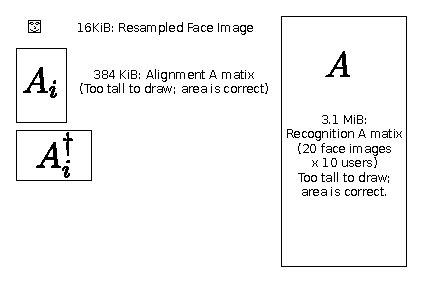
\includegraphics[scale=1.2]{figures/arrays}
	\label{fig:arrays}
}
\subfigure[The caches on a E5530 CPU]
{
	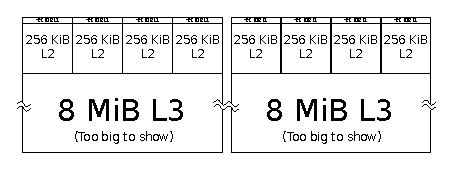
\includegraphics[scale=1.2]{figures/cpu_caches}
	\label{fig:cpu_caches}
}
\subfigure[The caches on a GTX480 GPU]
{
	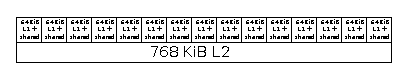
\includegraphics[scale=1.2]{figures/gpu_caches}
	\label{fig:gpu_caches}
}
\label{fig:caches}
\caption{A visual comparison of the algorithm working set to the CPU and GPU
caches.  Note: Although the aspect ratio could not be preserved, all arrays and
caches are drawn so that the area is proportional to the size of the data. } \vspace{-0.1in}
\end{figure}

% CPU CACHE DISCUSSION
%2MB = 2**21 bytes
%64*64*4 = 2**14 bytes = 16384 bytes per image
%... so can fit 2**7  = 128 images.
Each core has a private 32\,KiB L1 data cache and a private 256\,KiB L2 cache.
%16MB = 2**24 bytes = 16777216 bytes
%64*64*4 = 2**14 bytes = 16384 bytes per image
%... so can fit 2**10  = 1024 images.
Each processor further has 8\,MiB of L3 cache that is shared by the four cores.
Overall, the algorithm has approximately 16\,MiB of L3 cache
available for a dual-processor configuration.  

For floating-point instructions, each core also has a vector processing unit
(SSE) capable of performing the same arithmetic operation on four single-precision 
floating point values simultaneously.
There are thus two important levels of concurrency that need to be exploited to
efficiently use a modern CPU: {\em core-level} concurrency and {\em SSE-level}
concurrency. 

\subsection{GPU Hardware Concurrency} \vspace{-0.05in}
The main defining characteristics of contemporary multi-core GPU architectures
are that they have two (much wider) levels of concurrency, relatively small amounts of
 cache, and relatively low clock speeds.  Whereas most of the transistors on
a typical CPU are dedicated either to cache or to hardware that enables higher
clock speeds (such as branch prediction, out-of-order instruction execution, etc...),
most of the transistors on a GPU are dedicated to arithmetic logic units.
For our GPU implementations, we target NVIDIA Fermi GPU architecture (\eg, the GTX 480
GPU used in this paper).  An explanation of the GPU programming model (CUDA) at a useful level of completeness would take more space than is available here, so we will instead frame our discussion in terms of 
hardware capabilities. 
%\footnote{A discussion of the CUDA programming model can be found in the NVIDIA C for CUDA Programming Guide}
CUDA programmable GPUs are comprised of several
\emph{streaming multiprocessors} (SMP), each of which is roughly analogous to a CPU core.
For Fermi architecture GPU's, there are up to 16 SMP's, and each SMP is capable of executing up to 64 single precision 
floating point operations
concurrently. \footnote{In CUDA terms, the warp width is 32, and the floating pipeline can
issue up to two warps simultaneously}

% GPU CACHE DISCUSSION
% for L2 cache
% 768KB = 786432 bytes
% 64*64*4 = 2**14 bytes = 16384 bytes per image
% 48 images
Each SMP contains its own L1-cache, which is divided between hardware managed
and software managed ("shared") memory.  Additionally, all SMPs share a common
L2-cache.  For our system, each SMP has 64 KiB of L1 cache, and all SMP's share
768KB of L2 cache. 
%The cache hierarchy 
The relatively small amount
of cache (1/23 as much as CPU L3) on the GPU is balanced by a significantly
higher bandwidth between the processor chip and off-chip memory (DRAM) compared
to the CPU.  A scale drawing of the caches available on the GPU can be seen in Figure \ref{fig:gpu_caches}.
The GPU has its own memory system, and any data the GPU uses must first be
transferred from CPU DRAM to GPU DRAM over PCI-Express.  For our application,
this transfer overhead can be amortized over a large amount of computation and is
not a major concern.

While the programming model for
the SIMD units of each SMP is somewhat more flexible than on the CPU,
leveraging the flexibility typically comes at the cost of reduced concurrency.\footnote{
In CUDA terms, code branches that cause warp divergence usually
result in serialization of the different groups of threads}  Therefore, for
the purposes of comparing hardware architectures, the SIMD units on the GPU are
roughly analogous to the CPU SIMD units. Thus, in summary, the GPU hardware 
provides two levels of concurrency: {\em SMP-level}
concurrency and {\em thread-level} concurrency.  Note that the GPU provides more
concurrency than a CPU at both levels (14 SMP's vs. 8 cores) and (64 wide vs. 4 wide SIMD
units).


\section{Parallelism in the Face Alignment Stage}\vspace{-0.05in}
\label{sec:alignment}

Given the hardware concurrency in modern parallel computing architectures,
next, we shall study the optimal mappings of the algorithm parallelism in face
recognition to the multi-core CPUs and GPUs, respectively.  In this section, we
first focus on the face alignment stage (see Figure \ref{fig:pipeline}).

Face alignment \eqref{eq:l1min_alignment} estimates an image transformation
$\tau$ that rectifies the query image $\tilde{\bb}$ with possible pose
variation w.r.t. each training class $A_i$, which leads to the minimal sparsity
in error $\ee$ after the alignment. Note that directly solving
\eqref{eq:l1min_alignment} is inefficient since it is a non-convex problem
and may exhibit local minima.
However, given a good initial guess of the
transformation $\tau$ (\eg, provided by an accurate face detector), the optimal
solution for $\tau$ can be sought iteratively by linearization at each $j$th
step:
\begin{equation}
\min_{\xx, \ee, \Delta \tau_j}\|\ee\|_1\quad \subj\quad \tilde\bb\circ\tau_j +  J_j\Delta \tau_j = A_i\xx + \ee,
\end{equation}
where $J_j = \nabla_{\tau_j}(\tilde\bb\circ\tau_j)$ is the Jacobian, and
$\Delta \tau$ is a step update to $\tau$. Denote $\bb_j =
\tilde\bb\circ\tau_j$, $B_j = [A_i, -J_j]$ and $\ww^T = [\xx^T, \Delta
\tau^T]$, then the update $\Delta \tau$ can be computed by solving the
following linear program:
\begin{equation}
\min_{\ww, \ee}\|\ee\|_1\quad \subj\quad \bb_j = B_j\ww + \ee.
\label{eq:alignment-linearization}
\end{equation}
%If the warping $\tau$ is constrained to be a similarity transform,
%it can be paramaterized in such a way that the computation of $\frac{\partial \bb}{\partial \tau_p}$
%reduces to several linear vector operations involving pixel coordinates $(u,v)$, $\tau \in \Re^4$,
%and the image gradients $\f_x, \f_y \in \Re^M$, the latter of which only has to be computed
%once per test image.  
The per-class alignment algorithm via ALM is summarized in Algorithm
\ref{alg:iterative_alignment}. 
%In terms of computational complexity, one significant
%term is the computation of the matrix pseudo-inverse $B_j^\dagger$, whose
%computational cost is bounded by $O(n_i^2m + n_i^3)$. However, for per-class face
%alignment, since both $B_j$ and $J_{j}$ are very tall matrices (\ie, $m\gg n_i$
%for all $i=1, \cdots, K$ classes), we find that the computation cost is still
%dominated by the frequently computed matrix-vector multiplications in the
%inner loop.
\begin{algorithm}[ht!]
\caption{\bf (Face Alignment via ALM)} \label{alg:iterative_alignment}
\small
{\bf Input:} $\bb$, $A_i$, $\x_0 = \mathbf{0}$, $\tau_0$, and $J_0$.
\begin{algorithmic}[1]
\WHILE{not converged ($j = 1,2,\ldots$)}
\STATE Update $\bb_j \leftarrow \frac{\bb\circ \tau_{j-1}}{\|\bb\circ \tau_{j-1}\|}$; $B_j= [A_i, -J_{j-1}]$ and corresponding $(B_j^\dagger)^T$
\STATE Initialize $\ww_0 = \mathbf 0$, $\yy_0 = \mathbf 0$
\WHILE{not converged ($k = 1,2,\ldots$)}
\STATE $\uu_0\leftarrow \ww_{k-1}$; $\zz_0\leftarrow \ee_{k-1}$
\WHILE{not converged ($l = 1,2,\ldots$)}
\STATE $\zz_l \leftarrow \mbox{shrink}\left(\bb_j - B_j\uu_{l-1} + \frac{\yy_{k}}{\mu_{k-1}}, \frac{1}{\mu_{k-1}}\right)$
\STATE $\uu_l \leftarrow B_j^\dagger \left(\bb_j - \zz_{l} + \frac{\yy_{k-1}}{\mu_{k-1}} \right) $
\ENDWHILE
\STATE $\ww_k \leftarrow \uu_l$; $\ee_k \leftarrow \zz_l$
\STATE $\yy_{k} \leftarrow \yy_{k-1} + \mu_{k-1} (\bb_j - B_j\ww_{k} - \e_{k})$
\STATE $\mu_{k} \leftarrow \rho\mu_{k-1}$
\ENDWHILE
\STATE Update $\ee_j$, $\tau_j$, and $J_j$
\ENDWHILE
\end{algorithmic}
{\bf Output:} $\tau_i^*\leftarrow \tau_j, \e_i^*\leftarrow \ee_j$
\end{algorithm}

In summary, the alignment stage essentially contains two levels of available
parallelism. At the higher level, there are per-class alignment problems
that are solved independently, or \emph{problem-level parallelism}.  At a lower
level, the first-order linear algebraic operations exhibit parallelism within
image operations, \ie, at the pixel level.  We call this \emph{pixel-level
parallelism}.  The following two sections discuss methods for exploiting
these two levels of parallelism on CPU and GPU architectures.

\subsection{CPU Implementation} \vspace{-0.05in}
\label{sec:alignment_implementation_cpu}

Optimal implementation of Algorithm \ref{alg:iterative_alignment} on a multi-core CPU must take 
into account the properties of the cache hierarchy. In general, cache that is 
closer to the core (i.e. L1 cache) has higher bandwidth, but smaller size compared to cache
that is farther from the core (L3 cache).  For reference, Figure \ref{fig:cpu_caches} 
shows the the sizes of L2 and L3 caches of the Intel E5530 CPU, 
which is a representative example of a modern multi-core CPU. 

For the E5530, the L2 cache in each core is only able to store about 16 images.
For image alignment problem, the number of training images per class is
typically larger than 16.  
In this paper, we compare two mappings of the parallelism available in the alignment
stage to the concurrency available on the CPU: a naive implementation that is purely 
based on stock libraries and compilers, and a manually optimized version we advocate.

The naive implementation disregards 
problem-level parallelism, and instead maps pixel-level parallelism
onto both the core-level and the SSE-level concurrency provided by the CPU.  In
other words, alignment of the query image is performed
against a single subject at a time using all available cores on
the processors.  The potential advantage of this implementation is that all of the variables
for the inner loop, most notably $B_j$ and $B_j^\dagger$, fit in L2 cache.  

In contrast, our manually optimized implementation maps problem-level parallelism onto core-level
concurrency, and maps pixel-level parallelism onto SSE-level concurrency.  In
other words, eight instances of \eqref{eq:alignment-linearization} are executed
in parallel with each problem running on one of the eight cores.  The advantage
of this implementation is that since the cores are operating on different
alignment problem instances, no data is shared between cores, and therefore no
synchronization is necessary between the cores.  Furthermore, even with eight
problem instances running concurrently, the local variables for the inner
loop still fit in L3 cache.  Because of the sequential data access patterns of
the solver, the CPU hardware is able to use the full L3 cache bandwidth, which is 
high enough to make the program CPU limited, rather than memory limited.  
For these reasons, this implementation outperforms the previous naive solution.

%The implementation of some
%previous works \cite{WagnerA2009-CVPR,WagnerA2011-PAMI} are indeed based on the latter
%parallelization strategy.

%64 byte cache line-size per clock.  L3 cache running at lower clock than cpu.  Two reads and a write per clock.
%4 floats at a time in SSE.

In both implementations, most of the operations take
advantage of Intel Math Kernel Library (MKL), a commercial implementation of
the standard Basic Linear Algebra Subprograms (BLAS). For the image resampling
step, we make use of the Intel Integrated Performance Primitives (IPP) library.
Both MKL and IPP are optimized for Intel multi-core CPUs, and are able to
automatically utilize both core-level and vector-level concurrency (for the first implementation),
but are also available in single-threaded versions (for the second implementation). For 
operations that are not optimized by Intel in-house libraries, such as the shrinkage
operator in step 7 of Algorithm \ref{alg:iterative_alignment}, we achieve 
vector-level concurrency via
the automatic vectorization facilities of the Intel C++ compiler (ICC) \cite{dulong1999overview}.
To achieve core-level concurrency we make use of the Open MP API. \cite{dagum2002openmp} 
%We shall compare the performance of the two parallelism methods in Section \ref{sec:experiment}.

\subsection{GPU Implementation} \vspace{-0.05in}
\label{sec:alignment_implementation_gpu}
While on the CPU, algorithm performance is highly dependent on effective
cache usage, cache is relatively unimportant on the GPU for ALM based
$\ell_1$-min.  As can be seen in Figure \ref{fig:caches}, the GPU has 
a very small amount of cache compared to the CPU.  While it might be possible
to fit a single instance of the alignment problem (with a slightly reduced problem size)
into L2 cache, this would not be an efficient use of the GPU's resources.
The strength of the GPU's memory architecture for our purposes is its ability to sustain a very
high bandwidth to DRAM.  This bandwidth is achieved by having a very large number of
threads issuing interleaved memory requests.  Solving many alignment problem instances
concurrently increases the number of threads that can be used.

Therefore, our recommended GPU implementation is strikingly similar in spirit
to our recommended CPU implementation: on the CPU we use the cores to solve
multiple instances concurrently, and on the GPU we use multiple SMP's for the 
same purpose.\footnote{In CUDA terms, our proposed alignment stage
implementation consists of a single kernel that performs alignment for all
subject classes.  Each instance of the alignment problem is assigned its own
thread block, and the GPU hardware schedules as many thread blocks to run
concurrently as the hardware will allow.} The number of subject classes that
are actually scheduled to run concurrently is chosen by the GPU hardware, 
but can be indirectly influenced by manual tuning of the code (i.e., the kernel launch
configuration in CUDA terms). We have empirically determined
that performance is highest with 5-7 subject classes aligned simultaneously on each SMP.
%This mapping of the problem-level parallelism onto the SMP-level
%concurrency is illustrated in Figure \ref{fig:alignment_mapping_gpu}.
%\begin{figure}
%\centering
%
\includegraphics[width=3.4in]{figures/alignment_mapping_gpu}
%\caption{Proposed mapping of alignment parallelism onto GPU concurrency}
%\label{fig:alignment_mapping_gpu}
%\end{figure}

Several other aspects of the implementation merit discussion.  
First of all, we take advantage of the GPU's special hardware dedicated to bilinear interpolation
for the computation of $b(\tau)$ and $J(\tau)$, which essentially consist of resampled
versions of the test image and its derivatives.
Second, since there are no standard CUDA libraries that work at the SMP level, we use a
custom routine for computing $B_j^\dagger = (B_j^TB_j)^{-1} B^T = G^{-1} B_j^T$, with $G$
inverted using Gaussian elimination with partial pivoting.  To achieve
precision comparable to the single precision LAPACK routines in Intel's MKL
with this simplistic algorithm, we use double precision.  Since $G$ is only $n
\times n$ and $B_j^\dagger$ is only computed once per optimization problem, the
cost of the inversion is dwarfed by the cost of other steps.  
Similarly, sums and dot-products of large vectors are also
performed in double precision.
%The lack of a atomic floating point addition on the GPU
%significantly reduces the perfomance of this step of the algorithm.
%In Section \ref{sec:experiment}, we show the performance of our CPU and GPU
%implementations running on synthetic and real image data.

\section{Parallelization of the Face Recognition Stage} \vspace{-0.05in}
\label{sec:recognition}
After the face alignment stage is complete, the 20 subject classes with lowest
alignment error are selected for recognition, $\bb$ and $A_i$ are re-sampled to a common alignment
using $\tau_i$, and $A_i$ are concatenated into a new matrix $A$.
A sparse representation of $\bb$ w.r.t $A$ is then recovered
by solving a single $\ell_1$-min problem, as shown
in \eqref{eq:l1min_denoise}, using Algorithm \ref{alg:alm_rec}.  The
coefficients $\x$ are then used to compute error residuals that are used for
classification.  
%This recognition algorithm has
%been extensively studied in
%\cite{WrightJ2009-PAMI,YangA2010-ICIP,WagnerA2011-PAMI}.
In this stage of the algorithm, there is no problem-level
parallelism to exploit, so this section will discuss how to exploit pixel-level parallelism
on both CPU and GPU hardware.
Then in Section \ref{sec:experiment}, we will benchmark the
performance of the two architectures and further demonstrate the speed
gains achieved by our proposed implementations over previously published implementations.

\begin{algorithm}[t]
\caption{\bf (Face Recognition via ALM)} \label{alg:alm_rec} 
\begin{algorithmic}[1]
\begin{small}
\STATE {\bf Input:} $\bb \in \Re^m$, $A \in \Re^{m \times n}$,
$\x_1 = \mathbf{0}$, $\e_1 = \bb$, $\y_1 =
\mathbf{0}$.
\WHILE{not converged ($k = 1,2,\ldots$)}
\STATE $\e_{k+1} = \textup{shrink}(\bb - A\x_k +
\frac{1}{\mu}\y_k, \frac{1}{\mu})$;
\STATE $t_1\leftarrow 1$, $\z_1 \leftarrow \x_k$, $\w_1 \leftarrow \x_k$;
\WHILE{not converged ($l = 1,2,\ldots$)}
\STATE $\w_{l+1} \leftarrow \textup{shrink}(\z_l +
\frac{1}{\gamma}A^T(\bb - A\z_l - \e_{k+1} +
\frac{1}{\mu}\y_k), \frac{1}{\mu\gamma})$;
\STATE $t_{l+1} \leftarrow \frac{1}{2}( 1 +
\sqrt{1+4t_l^2})$;
\STATE $\z_{l+1} \leftarrow \w_{l+1} + \frac{t_l - 1}{t_{l+1}}(\w_{l+1} - \w_l)$;
\ENDWHILE
\STATE $\x_{k+1} \leftarrow \w_{l}$,  \; $\y_{k+1} \leftarrow \y_k + \mu (\bb - A\x_{k+1} - \e_{k+1})$;
\ENDWHILE \STATE
{\bf Output:} $\x^* \leftarrow \x_k, \e^* \leftarrow \e_k$.
\end{small}
\end{algorithmic}
\end{algorithm}

\subsection{Recognition Stage Implementation} \vspace{-0.05in}
Compared to problem-level
parallelism, the exclusively pixel-level parallelism in Algorithm \ref{alg:alm_rec} is
relatively straightforward to exploit:  
On the CPU, most of the operations map
well onto MKL BLAS calls, and operations that do not can be easily
parallelized using OpenMP and auto-vectorization.

On the GPU, most of the operations map well onto similar calls in NVIDIA's GPU
BLAS library (CUBLAS) which, like MKL, can take advantage of both levels of
concurrency available in the hardware architecture.  Operations that do not map
well onto the CUBLAS API were implemented directly in CUDA code.
Additionally, some operations that could have been implemented via multiple
BLAS calls, performance improvements were achieved by combining multiple
vector-vector operations into a single kernel, due to reduced bandwidth and
kernel call overhead.  

In order to avoid expensive data transfer across the bus connecting the GPU
card and the CPU motherboard (the PCI express bus), all of the data is
transferred to GPU DRAM once, and all non-trivial tasks are performed on the
GPU on data stored in GPU DRAM.  
%with the sole exception of the pseudo-inverse of $B_j$,
%which is computed on the CPU via Intel's LAPACK implementation, and then
%uploaded to GPU DRAM.  

\section{Experiments} \vspace{-0.05in}
\label{sec:experiment} 
In this section, we benchmark the
performance of our parallel implementations of $\ell_1$-min on CPU and GPU
platforms.  In order to show how our $\ell_1$-min algorithms scale with problem
size, in Section \ref{sec:simulation} we will begin with benchmarks for the
general $\ell_1$-min problem on synthetic data.  We will then progress in
Section \ref{sec:benchmark} to demonstrating the speed and accuracy of our
implementations as applied to the alignment and recognition stages of the face
recognition problem.
%To generate a meaningful comparison between different hardware architectures,
%in all cases we compare the performance of hardware architectures on a
%per-board basis:  For CPU implementations, the benchmark makes use of all of
%the cores in as many CPU's are present.  For GPU implementations, the benchmark
%makes the best use of the entire GPU chip (most GPU boards have a single GPU
%chip).  

\subsection{Simulations on Random Data}
\label{sec:simulation}

The first experiment compares the performance of our proposed CPU and GPU
implementations of the general $\ell_1$-min solver (Algorithm \eqref{alg:alm}).
The $d \times n$ measurement matrix $A$ is a random Gaussian matrix, with each
entry generated from the standard normal distribution and normalized to unit
column norm.  The ratio of $d/n$ is fixed at $1/2$ with $n$ varying from 1000 to 8000.
The ground truth signal, $\xx_0$ has a sparsity rate of 10\% of d with
elements sampled from a normal distribution and normalized to unit column
norm.  Because the ground truth signal $\xx_0$ is known, the algorithm
terminates when $\|\bx-\bx_0\| < \tau$ with $\tau=10^{-3}$.  The measurement
vector is generated by $\bb = A \xx_0$.   

The results of this benchmark can be found in Figure \ref{fig:random_data}.
The $x$-axis represents the size of the $A$ matrix and the $y$-axis represents the
average amount of time to complete a single problem instance.  The GPU
implementation tends to be faster than the CPU implementation at solving a
single large problem, whereas the CPU implementation is faster at solving a
single small problem.  The transition between the two regimes occurs (at 2000) where
the problem size begins to exceed the size of the CPU L3 cache. 
\begin{figure}
\begin{center}
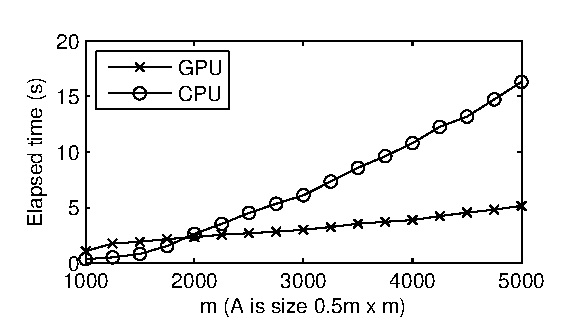
\includegraphics[width=2.5in]{figures/time_vs_matrix_size_constant_tol}
\end{center} \vspace{-0.1in}
\caption{\small Comparison of $\ell_1$-min runtime vs. dimensions of $A$ on random data.} \vspace{-0.1in}
\label{fig:random_data}
\end{figure}

\subsection{Face Recognition Pipeline Benchmark} \vspace{-0.05in}
\label{sec:benchmark}
This section presents benchmarks of the CPU and GPU implementations of the
alignment stage (i.e., Algorithm
\ref{alg:iterative_alignment}) as well as the recognition stage (i.e., Algorithm \ref{alg:alm_rec}) of the
face recognition pipeline.

First, in order to measure the impact of solving many
$\ell_1$ problems-per concurrently on the GPU, we benchmark three implementations of the
alignment $\ell_1$-min solver with $A$ of size $5120 \times 32$, and a fixed
$50$ inner loop iterations for each of $50$ outer loop iterations. The runtime
on a GTX480 GPU is averaged over a large number of trials, which are run
sequentially or concurrently depending on the implementation.
The results are shown in Table \ref{tbl:ubench}.
Our proposed parallelization of the $\ell_1$-min used in the alignment
stage is {\em eight times} faster than an implementation solving a single
problem at a time using the stock BLAS libraries.
\footnote{The streams implementation is limited significantly by a 
cap on the number of concurrent streams in the current version of CUDA}
%The results are shown below:
\begin{table}[t!]
\caption{\small Benchmark of implementations of alignment $\ell_1$-min.}
\small
\begin{tabular}{|l|c|}
\hline
Sequential solver using CUBLAS & 302\,ms \\
\hline
One problem per SMP using CUDA streams & 70\,ms  \\
\hline
Four problems per SMP using single kernel & {\bf 36\,ms} \\
\hline
\end{tabular} \vspace{-0.1in}
\label{tbl:ubench}
\end{table}
 
Using an implementation motivated by the previous result, we now benchmark our
iterative alignment implementation on real face data.  For experiments on face
data we use subsets of the CMU Multi-PIE Face Database.  For gallery images we
use frontal images from session 1, which contains 20 images per subject taken
under different illuminations. For test images we use images from session 2.
The training images are prepared as follows: The iterative alignment stage
seeks a similarity transformation between the coordinate frame of the
full-resolution test image and a ``canonical'' coordinate frame in which images
are compared.  The training images are aligned by applying a similarity
transormation that maps two manually clicked outer eye corners to fixed
locations in the canonical frame.  A $64 \times 64$
pixel window in the canonical frame is used for resampling. 

Figure \ref{fig:alignment_stage_runtime} shows the average run time of the CPU and GPU implementations to align
a query image against all the subject classes separately. We vary the total number of
subject classes to show how the algorithms scale. The plateaus seen in the GPU curve
result from the GPU hardware scheduling the computation of alignment
problems in concurrent batches, but the overall trend is linear as expected.
The manually threaded CPU implementation slightly outperforms the GPU implementation,
and it beats the \emph{naive}
library threaded implementation by a wide margin.
The new implementation can align the query
image in $\approx 40$ ms per subject, 
while the fastest previously published result \cite{WagnerA2011-PAMI}
required $\approx 600$ ms seconds per subject in a similar setting.  

\begin{figure}[t!]
\centering
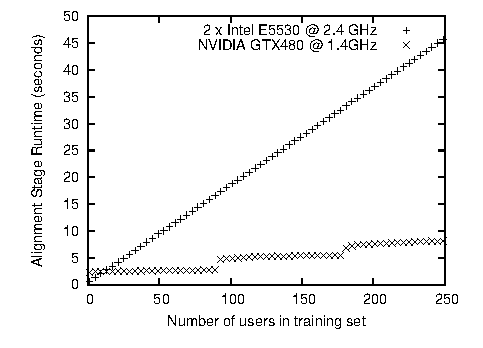
\includegraphics[width=3.3in]{figures/alignment_runtime_graph}\vspace{0.05in}
\caption{Alignment stage runtime vs. size of training database.} \vspace{-0.1in}
\label{fig:alignment_stage_runtime}
\end{figure}

The next experiment compares the speed of the GPU and CPU implementations of
the recognition stage.  It was determined that keeping 20 gallery subjects is
sufficient to ensure that the correct subject is kept for the recognition stage
with 95\% probability.  Since recognition failures are typically caused by a
poor alignment, we find that keeping more subjects for the recognition stage does
not necessarily improve recognition rate.

Figure \ref{fig:recognition_stage_runtime} shows the recognition stage runtime
for canonical images of size: $32\times32$, $48 \times 48$, $64 \times 64$, $96 \times
96$, and $128 \times 128$.  For all image resolutions, the problem size
is sufficiently small that the CPU is significantly faster than the GPU.  Note
also that for both implementations, the recognition stage takes much less time
than the alignment stage.
\begin{figure}[t!]
\centering
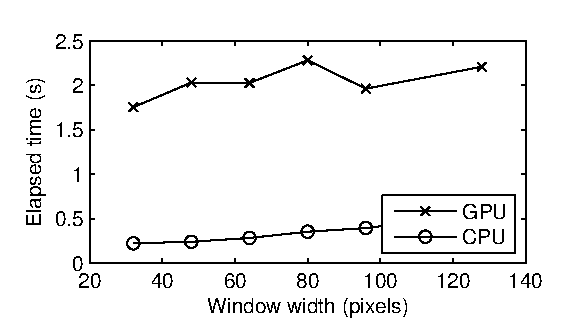
\includegraphics[width=2.5in]{figures/speedVsResolution} \vspace{-0.05in}
\caption{Recognition stage runtime vs. face window resolution}\vspace{-0.1in}
\label{fig:recognition_stage_runtime} \end{figure}

Finally, we perform an experiment verifying the recognition accuracy of the
overall pipeline.  As shown in Figure \ref{fig:accuracy_vs_resolution},
at the optimal resolution, which happens to match the alignment stage
resolution, the GPU implementation reaches 95\% recognition rate, the max
achievable given the alignment selection process.  For significantly lower resolutions,
the accuracy drops off significantly.  The slight difference in CPU vs. GPU
accuracy may be a result of numerical precision differences in our matrix
inversion and vector reduction routines.
\begin{figure}[t!]
\centering
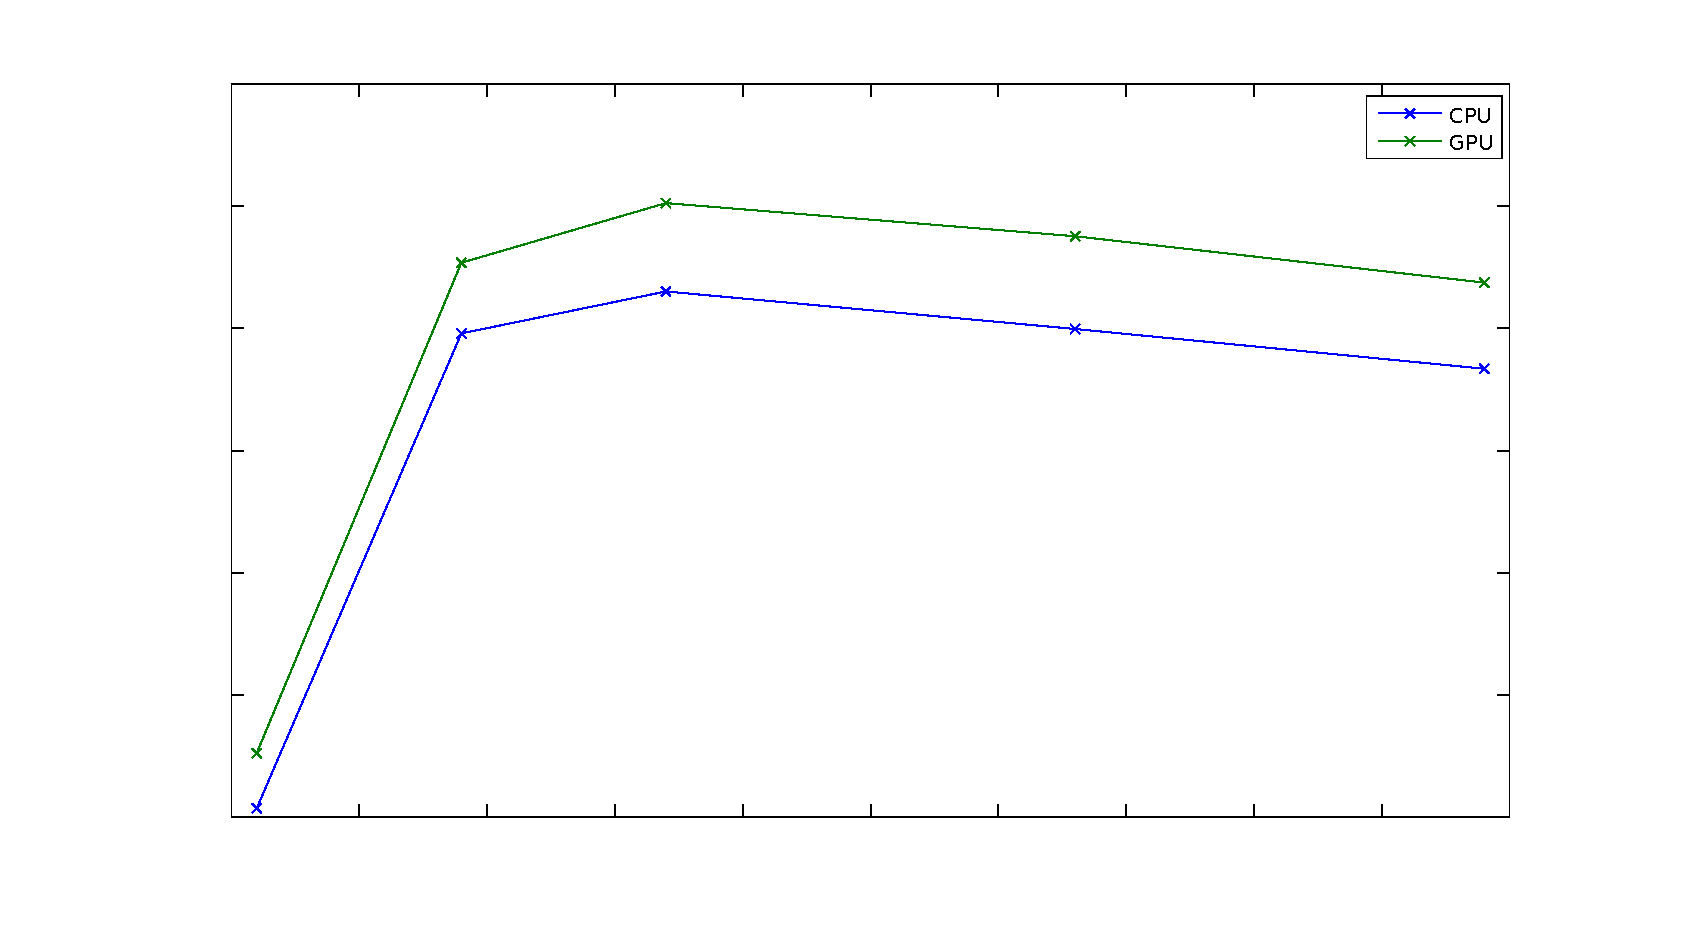
\includegraphics[width=2.5in]{figures/accuracyVsResolution} \vspace{-0.05in}
\caption{Recognition rate of the full pipeline vs. face window resolution.} \vspace{-0.1in}
\label{fig:accuracy_vs_resolution}
\end{figure}

\section{Conclusion}\vspace{-0.05in}
We have demonstrated that on both CPU and GPU algorithms, parallelizations of
ALM that solve multiple face alignment problems concurrently are significantly
faster than implementations that rely purely on vendor-supplied BLAS libraries.
Furthermore, thanks to a combination of faster hardware, and more efficient use
of the hardware, we have demonstrated dramatic improvements in recognition
speed over previously reported implementations.
As CPU manufacturers increase the number of cores and vector widths, and as GPU 
manufacturers increase the amount
of cache, both architectures are rapidly converging towards an architectural balance
that increasingly favorable for $\ell_1$-min based face recognition.
% of the same pipeline.  Whereas
%earlier implementations required over a second to align a test image against
%just one of the 250 subjects in Multi-PIE session 1, the proposed 
%implementations can perform the same task in 
%{\bf under 10 seconds}!.  
%The parallelization techniques presented here make it feasible to implement an
%access control system for hundreds of subjects on a handful of purpose-build
%multi-GPU workstations.  


%We argue that in addition to vendor supplied libraries
%that attempt to leverage both levels of concurrency of the GPU, there is a need
%for standard libraries that operate at the SMP level of concurrency.

{\small
\bibliographystyle{ieee}
\bibliography{faces-short}
}

\end{document}

